\chapter{Application Development Plan}

A visualization for the plan for this project can be seen in the Gannt chart in figure \ref{fig:gannt}
\begin{figure}
	\caption[Gannt Chart of the Project]{Gannt chart showing the project's planned process over the academic year.}
	\label{fig:gannt}
	\begin{center}
	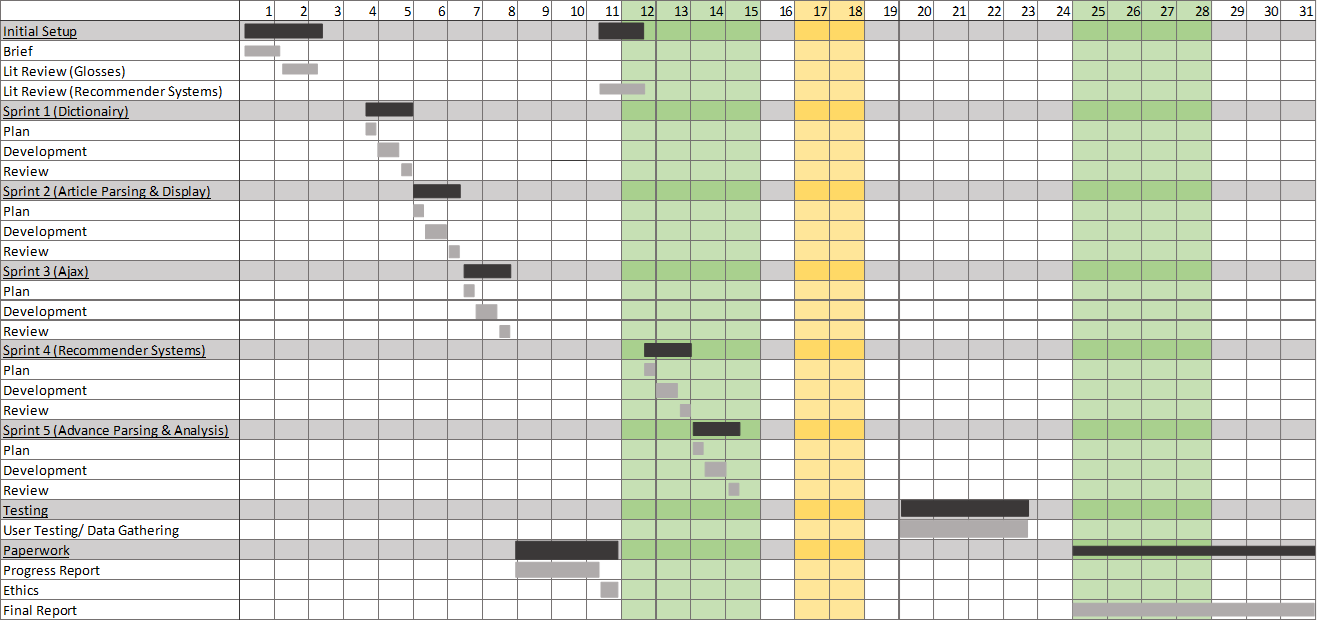
\includegraphics[width=\textwidth]{Graphics/Gannt}
	\end{center}
\end{figure} 

\section{Readings and Research}

The plan details that reading was to be divided into two parts, reading about glosses and reading about difficulty rating systems. With the reading about difficulty rating systems being done after the gloss was developed. This was done as the difficulty rating system was not part of the minimum viable project, so the reading about it could be left until after the development of the minimum viable project was complete.

\section{Development}

The application was developed using AGILE methods. The project was divided into six sprints and they were completed in the order in which they are described. The order was chosen as it would allow the application to reach minimal viable project status as soon as possible (end of sprint 3), leaving the more advanced sprints for later. The sprints are detailed below.

\begin{enumerate}
	\item \textbf{Translation Lookup}
	
	The aim of this sprint is to establish a valid method to retrieve single word translation and grammatical data.
	
	\item \textbf{Article Parsing \& Presentation}
	
	The aim of this sprint is develop a method for the parsing of articles and then to present them through a web browser
	
	\item \textbf{AJAX}
	
	The aim of this sprint is to develop the javscript code that will allow the gloss to display entries.
	
	\item \textbf{Advance Parsing}
	
	The aim of this sprint is to allow advanced parsing methods to be performed on the text. Allowing for parts of speech identification of words. 
	
	\item \textbf{Article Discovery}
	
	The aim of this sprint is get the application to find articles on it's own, removing the need for the user to find their own articles.
	
	\item \textbf{Difficulty Rating System}
	
	The aim of this sprint it to develop the system that allows the application to rate how difficult the user will find various articles. 
	
\end{enumerate}

AGILE methodologies were used as they allowed the developer to have regular meetings with the project supervisor, discussing the progress made, what was left to be done whether or not it was achievable.

\section{Testing}

Three types of testing were done on the application. Unit testing was during the development of sprint one, to ensure that the application was interacting with the dictionary API correctly, making sure that the correct translations of various words were found. 

functional testing was during the development of the rest of the application, the developer would use the application, testing whether or not the feature they were currently implementing was working as planned.

Finally, user testing was done once all six sprints were completed, it consisted on the user using the application to read three articles, and then filling out a feed back survey about their experiences with it. In addition, the user's use of the application was tracked, seeing what words they requested and what articles they read. Ethics approval for this test was obtained from the ECS ethics board. 